%%%%%%%%%%%%%%%%%%%%%%%%%%%%%%%%%%%%%%%%%%%%%%%%%%%%%%%%%%%%%%%
% rjw 11/25/18 Make subsection of the Validation section 
%
\subsection{Simulation}
\label{sec:fdsp-pd-simphys}
%\metainfo{(Length: \dword{tdr}=50 pages, TP=20 pages)}
%\metainfo{\color{blue} Content: Conveners}
% Provided by Alex H. 15mar18
%\metainfo{Content: Himmel}

%Content update by AH nov 2018
%edits by rjw nov 2018

The detector requirements for the photon detection system are determined by a series of physics deliverables addressing the major physics goals of DUNE: nucleon decay searches, supernova burst neutrinos, and beam neutrinos. The system requirements then flow from the physics needs, determined using a full simulation, reconstruction, and analysis chain developed for the \larsoft framework. 
%The goal is to evaluate the performance in physics deliverables for each of the photon collector designs under consideration. The metrics evaluated will include efficiency for determining the time of the event ($t_0$), timing resolution, and calorimetric energy resolution for three physics samples: \dword{snb} neutrinos, nucleon decay events, %\footnote{The most relevant sample is actually the \emph{background} to nucleon decay events. However, efficiently simulating background that can mimic nucleon decays is challenging since they can be quite rare topologies, so it is easier to simulate the nucleon decay signal which should be representative of the background.}, 
%and beam neutrinos. However, the development of analysis tools to take advantage of this full simulation chain is fairly recent, so this proposal will only include one test case: $t_0$-finding efficiency for \dword{snb} neutrinos versus the effective area of the photon collectors (see Section~\ref{sssec:photoncollectors}).

\fixme{Need references to the Requirement/Specifications Tables in each subsection ideally}

\subsubsection{Description of Simulation and Reconstruction}

The first step in the simulation specific to the \dword{pds} is the simulation of the production of light and its transport within the volume to the \dwords{pd}. Argon is a strong scintillator, producing \SI{24000}{$\gamma$s/MeV} at our nominal drift field. Even accounting for the efficiency of the \dwords{pd}, it is prohibitive to simulate every optical photon with \dword{geant4} in every event. So, prior to the full event simulation, the detector volume is voxelized and many photons are produced in each voxel. The fraction of photons from each voxel reaching each photosensor is called the visibility, and these visibilities are recorded in a 4-dimensional library (akin to the photon maps used in the \dword{dpmod} simulation described in \voltitledp~Chapter 5.
\fixme{This reference to DP chapter 5 is hardwired - check this is the correct chapter number.}
% described in Section~\ref{subsec:fddp-pd-6.1.1}). 
% doesn't appear possible to reference a section in the other volume.
This library includes Rayleigh scattering length ($\lambda=$ \SI{60}{cm}\cite{Grace:2015yta}), absorption length ($\lambda=$ \SI{20}{m}), and the measured collection efficiency versus position of the double-shift light-guide bars. When a particle is simulated, at each step it produces charge and light. The light produced is distributed onto the various \dwords{pd} using the photon library as a look-up table and the 30\% early (\SI{6}{ns}) plus 70\% late (\SI{1.6}{$\mu$s}) scintillation time constants are applied. Transport time of the light through the \lar is not currently simulated, but is under development.

The second step is the simulation of the sensor and electronics response. For the studies shown here the SensL \dword{sipm} and \dword{sipm} signal processor (\dword{ssp}) readout electronics used for \dword{pd} development and in \dword{pdsp} is assumed (see Section~\ref{sec:fdsp-pd-pde}). However, a range of signal-to-noise and dark rates are considered in order to set requirements on the needed performance of the electronics.
%Waveforms are produced on each channel by adding an \dword{sipm} single-\phel response shape for each true photon. In addition, other characteristics of the \dword{sipm} are included such as dark noise, and crosstalk, based on data from device measurements. 
%) From Alex 4/17/18 - We do include afterpulsing as well, at rates based on the sensl sipm's tested in Hawaii. You can just add it to the list of things included in the electronics simulation. 
Crosstalk (where a second cell avalanches when a neighbor is struck by a photon generated internal to the silicon) is introduced by adding a second \phel \num{16.5}\% of the time when an initial \phel is added to the waveform. Additional uncorrelated random noise is added to the waveform with an RMS of %\SI{2.6}{ADC} (or approximately 
\SI{0.1}{\phel}. The response of the SSP self-triggering algorithm, based on a leading-edge discriminator, is then simulated to determine if and when a \SI{7.8}{$\mu$s} waveform will be read out, or in the case of the simulation it will be stored and passed on for later processing.

The third step is reconstruction, which proceeds in three stages. The first is a ``hit finding'' algorithm that searches for peaks on individual waveforms channel-by-channel, identifying the time based on the time of the first peak and the total amount of light collected based on the integral until the hit goes back below threshold. The second step is a ``flash finding'' algorithm that searches for coincident hits across multiple channels. All the coincident light is collected into a single object that has an associated time (the earliest hit), an amount of light (summed from all the hits), and a position on the plane of the \dwords{apa} ($y$-$z$) that is a weighted average of the positions of the photon collectors with hits in the flash. %\footnote{Currently, the flash reconstruction does not consider the positions of the hits, only their times. This will need to be updated in the future when we simulate the full-sized \dword{spmod} but for now we are working in a small test geometry that acts as a crude simulation of this kind of constraint.}. 
The final step is to ``match'' the flash to the original event by taking the largest flash within the allowed drift time that is within \SI{240}{cm} in the $y$-$z$ plane. Since the TPC reconstruction is still in active development, especially for low-energy events, we match to the true event %\dword{mc} 
vertex of the event in the analyses presented here. This is a reasonable approximation since the position resolution of the TPC will be significantly better than that of the \dword{pds}. 

These tools (or subsets of them) are then used to evaluate how the performance of the photon detection system affects the following set of physics deliverables.

\subsubsection{Nucleon Decay}

Nucleon decays are rare events, so excluding backgrounds is of the utmost importance. Since some backgrounds can be generated by cosmic rays passing outside the active detector area, setting a fiducial volume to exclude such events is critically important.

\textit{\it T0 for Fiducialization}

The physics deliverable: the photon detectors must be able to determine T0 with approximately \SI{1}{\micro s} resolution for events with visible energy greater than \SI{200}{MeV} throughout the active volume with high efficiency ($>99\%$). This energy regime is relevant for nucleon decay and atmospheric neutrinos. The time measurement is needed for event localization for optimal energy resolution and rejection of entering backgrounds. 
This time resolution is required for comparable spatial resolution to the TPC along the drift direction.

\begin{dunetable}[Photon detector efficiency for nucleon decay events]
{ccc}
{tab:pds-ndk}
{Efficiency for tagging nucleon decay events at the CPA (\SI{3.6}{m} from the photon detectors) with the photon detection system for a range of ``effective area'' (efficiency times active area) per module and the equivalent light yield per MeV at the CPA.}
Effective Area (cm$^{2}$) & Light Yield (PE/MeV) & Efficiency at the CPA \\ \toprowrule
4.1   & 0.09 & $93.8 \pm 0.4$ \\ \colhline
5.1   & 0.11 & $95.0 \pm 0.4$ \\ \colhline
7.4   & 0.16 & $96.8 \pm 0.4$ \\ \colhline
12.8  & 0.28 & $97.7 \pm 0.4$ \\ \colhline
15.0  & 0.33 & $98.4 \pm 0.2$ \\ \colhline
23.0  & 0.50 & $98.9 \pm 0.2$ \\ \colhline
\end{dunetable}


The physics here feeds down to a requirement on the efficiency of the photon detection system (equiv. light yield), determined by measuring how often the correct flash was not assigned to nucleon decay 
events\footnote{The most relevant sample is actually the \emph{background} to nucleon decay events. However, efficiently simulating background that can mimic nucleon decays is challenging since they can be quite rare topologies, so it is easier to simulate the nucleon decay signal which should be representative of the background.} 
vs. distance from the APA and vs. the efficiency of the photon detectors using the full simulation and reconstruction described in the previous section. The results of the simulation studies are shown in Table~\ref{tab:pds-ndk}. A light collector design that achieves \SI{23}{cm^2} effective area equivalent to a light yield of \SI{0.5}{PE/MeV}) meets the requirement of 99\% efficiency at the CPA (Table~\ref{tab:spec:light-yield}).


\subsubsection{Supernova Neutrinos}

Supernova bursts are also rare events, though here the `event' is made up of many interactions instead of a single interaction. For distant supernovas (at the far side of the Milky Way or in the Large Magellanic Cloud), the top priority is to ensure that the detector can identify a burst when it happens and trigger the readout of the detector. For nearby supernova triggering will not be a challenge, and instead the goal is to record as much information as possible about the burst.

\textit{\it Burst Triggering}

The physics deliverable: the photon detection system must be able to trigger on supernova bursts in our galaxy and the Large Magellanic Cloud with efficiency similar to the TPC, with a false positive rate of less than one per month. This deliverable is most important for distant supernova where the most important requirement is that we trigger and record the data. The PDS-based trigger should have similar performance to the TPC trigger so they can provide redundancy against one another or be combined to increase efficiency or lower the background rate. The once-per-month false positive rate is determined by limits from the DAQ and data handling.

\fixme{Results of the SNB triggering studies will go here when available}


\textit{\it T0 for TPC Energy Measurement and Time Resolution}

The physics deliverable: the photon detectors must be able to provide T0 determination with approximately \SI{1}{\micro s} resolution for at least 60\% of the neutrinos in a typical supernova energy spectrum. The T0's are used in concert with the TPC-reconstructed event in two ways: to correct for the attenuation of the charge signal as a function of how far the charge drifts through the TPC and to provide more precise absolute event times for resolving short time features in the supernova neutrino event rate. This deliverable is important primarily for nearby supernova where the number of events is large enough that time and energy resolution will be the limiting factors in extracting physics. 

\begin{dunefigure}[Supernova neutrino energy resolution for different PD performance assumptions.]
{fig:pds-snb-driftcor}
{The energy resolution for supernova neutrino events when reconstructed by the TPC and drift corrected with varying assumptions on the performance of the photon detectors. The options considered range from drift correction for no events (black), to 60\% of events (blue), to 100\% of events (red).}
  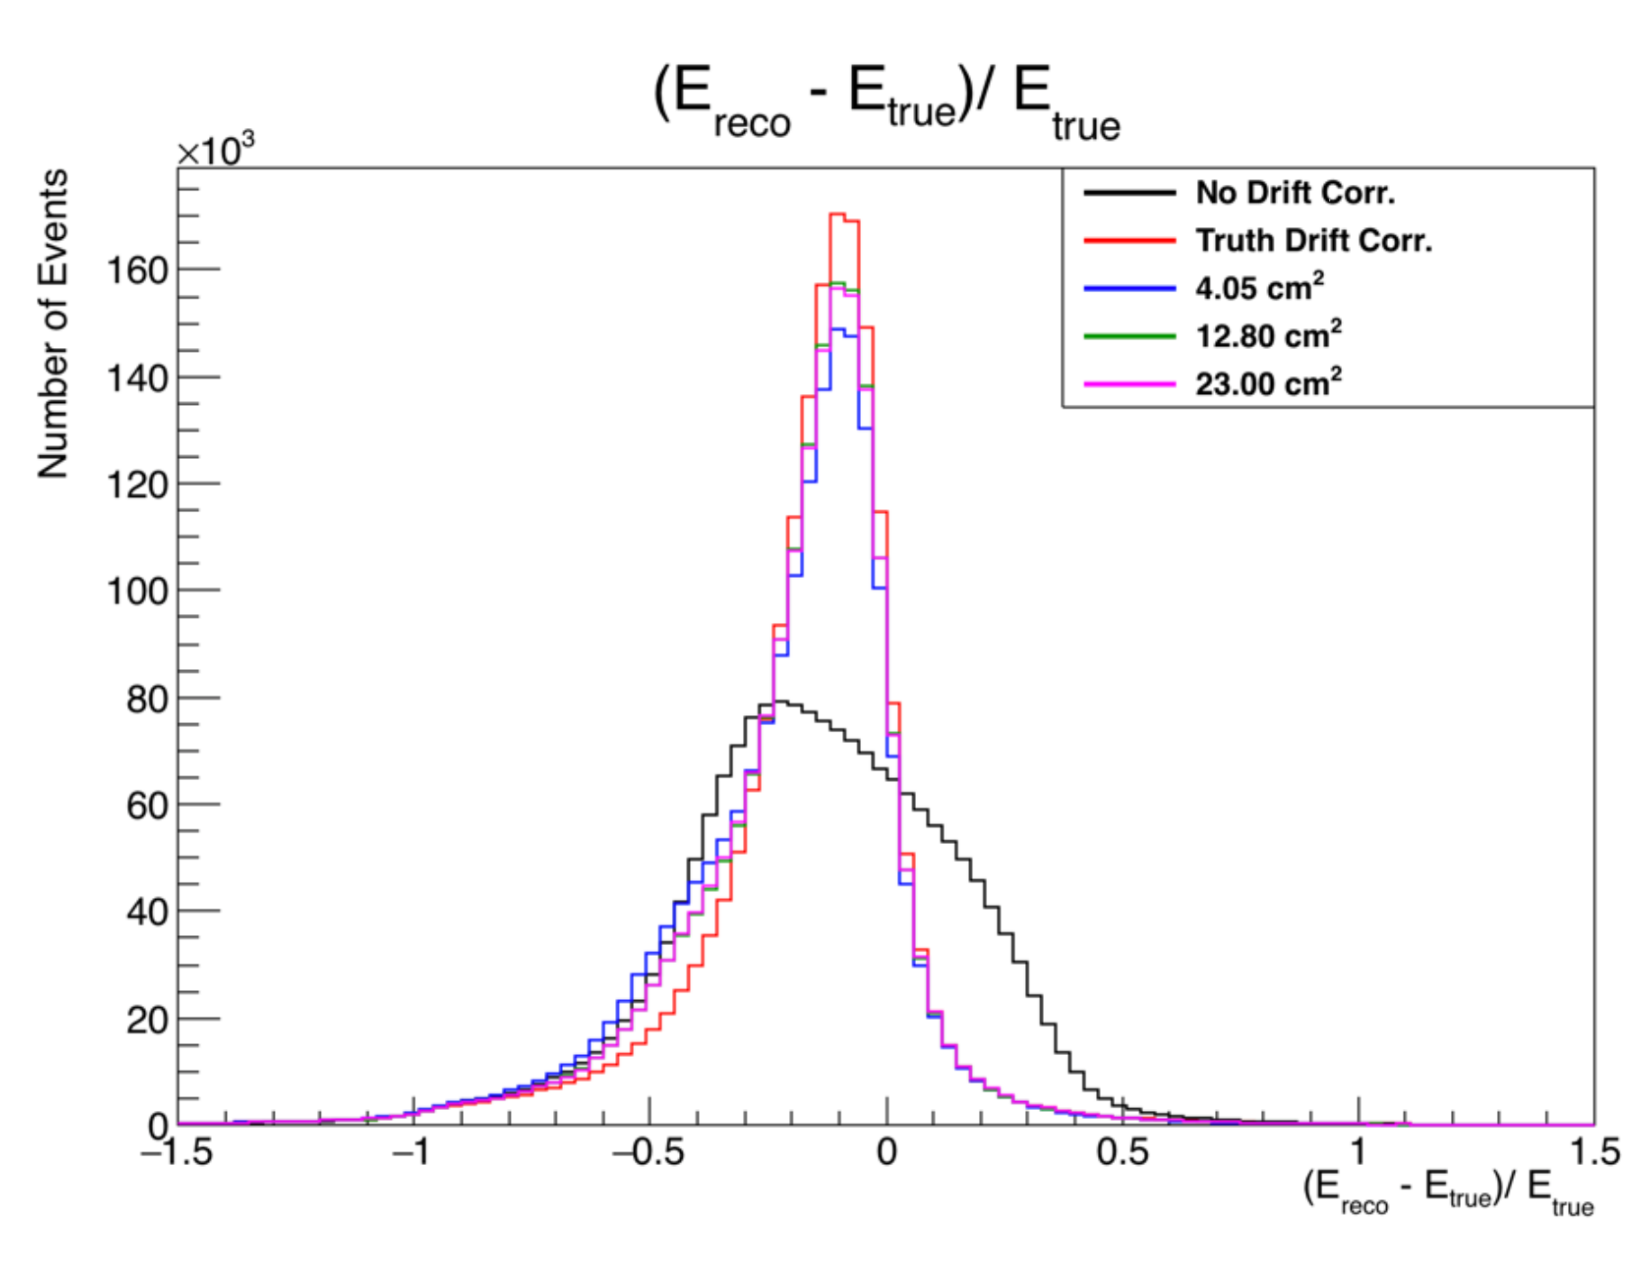
\includegraphics[width=0.4\columnwidth]{graphics/pd-snb-tpc-eres}
 \fixme{Larger text font on the plot so still legible when plot size reduced}
\end{dunefigure}

The 60\% T0 tagging requirement comes from two studies of a typical supernova neutrino spectrum under varying photon detector performance assumptions: the resolution of the energy reconstructed with the TPC and drift-corrected using the time from the photon detectors, and the observability of the in-fall `notch' in the supernova event time distribution. Both studies show significant improvement when going from no photon detectors to a system with an effective area of \SI{4.05}{cm^2} (equivalent to \SI{0.5}{PE/MeV} for 60\% of the detector volume), but only marginal improvements past that point. This sets a requirement on light yield, but other physics deliverable set more stringent requirements.


\textit{\it Calorimetric Energy}

Physics deliverable: the photon detection system should be able to provide a calorimetric energy measurement for low energy events, like supernova neutrinos, complementary to the TPC energy measurement. 
Improving the energy resolution, up to the fundamental limits imposed by invisible particles in the interaction, will enable us to extract the maximum physics from a supernova burst, and with the goal to achieve energy resolution comparable to the TPC, full advantage can be taken of the anti-correlation between the emission of light and charge signals imposed by the conservation of energy.

\fixme{Results of SNB calorimetry studies will go here}


\subsubsection{Beam Neutrinos}

The photon detection system is not needed for fiducializing beam neutrino events since the pulsed beam will provide sufficient precision to place the interactions in space. However, the photon detectors can potentially contribute to the energy measurement and the better timing resolution can help identify Michel electrons from muon and pion decay.


\textit{\it Calorimetric Energy}

Physics deliverable: the photon detection system should be able to provide a calorimetric energy measurement for high energy events, like neutrinos from the LBNF beam, complementary to the TPC energy measurement.
Neutrino energy is an observable critical to the success of the oscillation physics program, and a second independent measurement can provide a cross-check which reduces systematic uncertainties or directly improves resolution for some types of events. In order to provide a meaningful cross-check, the resolution and uncertainty of the photon detection system measurement must be comparable to the calorimetric resolution of the TPC. The limit on this measurement will likely come from how well the efficiency of the detectors and the optical properties of the argon can be determined (both must be known to approximately 5\% to have a comparable measurement of electron shower energy), which define a program of measurements between now and the operation of the detector rather than requirements on the system itself. The requirement that does flow down from this is that the dynamic range of the system is sufficient to allow for accurate measurement of the amount of light reaching the photon detection system. 

\fixme{Results of beam dynamic range studies will go here. TPC requirement is < 10\% of events saturate.}


\textit{\it Michel Electron Tagging}

Physics deliverable: the photon detection system should be able to identify events with Michel electrons from muon and pion decays.
The identification of Michel electrons can improve background rejection for both beam neutrinos and nucleon decay searches. 
Some Michel electrons are difficult to identify with the TPC since they appear simultaneous within the time resolution of the TPC and collinear with their parent. However, because the photon detection system can observe the fine time structure of events in the detector, they can identify Michel electrons that appear separated in time from the main event.

\fixme{Unlikely to have real studies here in time for even the second draft. Drop this requirement? Or can we use Lariat experience somehow?}


